%=================================================================
% CSE 4345 — Big Data Analytics
% Week 8, Part 1: Data Integration at Scale —
%                 Pipelines, Data Lakes, and Modern Architectures
% Department of CSE, Premier University
%
% Part 1 covers: Batch integration (Sqoop, Flume) · Apache Kafka log model
%               · Kafka architecture (topics, partitions, consumer groups)
%               · Lambda architecture (Marz) · Kappa architecture (Kreps)
%               · Data lake components · Ivy League alignment · Assessment
% Part 2 covers: Kreps et al. (2011) Kafka paper · Netflix pipeline case study
%=================================================================

\documentclass[aspectratio=169,10pt]{beamer}

%---------- Packages ----------
\usepackage[utf8]{inputenc}
\usepackage[T1]{fontenc}
\usepackage{booktabs}
\usepackage{xcolor}
\usepackage{tikz}
\usetikzlibrary{shapes.geometric, positioning, arrows.meta,
                decorations.pathreplacing, calc, fit, backgrounds}
\usepackage{amsmath}
\usepackage{graphicx}
\usepackage{multicol}
\usepackage{enumerate}
\usepackage{array}
\usepackage{listings}

%---------- Theme ----------
\usetheme{Madrid}

%---------- Premier University Color Identity ----------
\definecolor{PUNavy}{RGB}{10,36,99}
\definecolor{PUGold}{RGB}{197,151,37}
\definecolor{PULightBlue}{RGB}{210,228,255}
\definecolor{PUTeal}{RGB}{0,100,100}
\definecolor{PUGray}{RGB}{90,90,90}
\definecolor{PURed}{RGB}{160,30,30}
\definecolor{PUGreen}{RGB}{30,120,60}
\definecolor{PUOrange}{RGB}{200,100,20}
\definecolor{PUPurple}{RGB}{80,0,120}

\setbeamercolor{palette primary}{bg=PUNavy, fg=white}
\setbeamercolor{palette secondary}{bg=PUNavy!85, fg=white}
\setbeamercolor{palette tertiary}{bg=PUNavy!70, fg=white}
\setbeamercolor{palette quaternary}{bg=PUNavy, fg=white}
\setbeamercolor{structure}{fg=PUNavy}
\setbeamercolor{title}{bg=PUNavy, fg=PUGold}
\setbeamercolor{subtitle}{fg=white}
\setbeamercolor{frametitle}{bg=PUNavy, fg=PUGold}
\setbeamercolor{alerted text}{fg=PUGold!85!black}
\setbeamercolor{block title}{bg=PUNavy, fg=white}
\setbeamercolor{block body}{bg=PULightBlue!45}
\setbeamercolor{block title alerted}{bg=PUGold!80!black, fg=white}
\setbeamercolor{block body alerted}{bg=PUGold!12}
\setbeamercolor{block title example}{bg=PUTeal, fg=white}
\setbeamercolor{block body example}{bg=PUTeal!10}
\setbeamercolor{section in toc}{fg=PUNavy}
\setbeamercolor{itemize item}{fg=PUGold!80!black}
\setbeamercolor{itemize subitem}{fg=PUNavy!70}

\setbeamertemplate{navigation symbols}{}
\setbeamertemplate{itemize item}{\scriptsize\raise1.5pt\hbox{\textbullet}}
\setbeamertemplate{itemize subitem}{\scriptsize\raise1pt\hbox{--}}

%---------- Code listing style ----------
\lstset{
  basicstyle=\ttfamily\scriptsize,
  backgroundcolor=\color{PUNavy!8},
  frame=single,
  rulecolor=\color{PUNavy!30},
  breaklines=true,
  language={},
  keywordstyle=\color{PUNavy}\bfseries,
  commentstyle=\color{PUGray}\itshape,
  stringstyle=\color{PUGreen!70!black},
}

%---------- Section separator ----------
\AtBeginSection[]{
  \begin{frame}[plain]
    \vfill\centering
    \begin{beamercolorbox}[sep=12pt,center,shadow=true,rounded=true]{block title}
      \usebeamerfont{title}\insertsectionhead\par
    \end{beamercolorbox}
    \vfill
  \end{frame}
}

%---------- Title metadata ----------
\title[CSE 4345 \textbar{} Week 8, Part 1]{CSE 4345: Big Data Analytics}
\subtitle{Week 8, Part 1 \textemdash\ Data Integration at Scale:
  Pipelines, Data Lakes \& Modern Architectures}
\author[Dept.\ of CSE]{Department of Computer Science \& Engineering\\[4pt]
       \small Premier University, Chittagong}
\institute{}
\date{Semester 2026}

%=================================================================
\begin{document}
%=================================================================

%----------------------------------------------------------------
\begin{frame}
  \titlepage
\end{frame}

%----------------------------------------------------------------
\begin{frame}{Course \& Lecture Information}
  \begin{columns}[T]
    \column{0.47\textwidth}
      \begin{block}{Lecture Identity}
        \begin{tabular}{ll}
          \textbf{Course:}      & CSE 4345 \\
          \textbf{Week / Part:} & 8 of 11 \textbar\ Part 1 of 2 \\
          \textbf{CLO:}         & CLO3, CLO4 \\
          \textbf{PLO:}         & PLO(e), PLO(f) \\
        \end{tabular}
      \end{block}
      \vspace{6pt}
      \begin{alertblock}{CLO3 \& CLO4}
        \small \textbf{CLO3:} \textit{Explain big data techniques and tools to store, manage, and analyse large datasets}\\[4pt]
        \textbf{CLO4:} \textit{Solve big data problems and build a project applying big data tools and frameworks}
      \end{alertblock}
      \vspace{6pt}
      \begin{block}{Course Progression}
        \small
        Week 6: Spark, RDDs, in-memory computing\\
        Week 7: Hive, HiveQL, SQL-on-Hadoop\\
        \textbf{Week 8: Pipelines, Kafka, Lambda/Kappa}\\
        Week 9: Data visualisation and dashboards
      \end{block}

    \column{0.50\textwidth}
      \begin{exampleblock}{Part 1 Covers}
        \begin{itemize}
          \item From ETL to pipelines: the shift in integration thinking
          \item Data integration tool landscape (Sqoop, Flume, Kafka, NiFi)
          \item Apache Sqoop: bulk RDBMS $\leftrightarrow$ HDFS transfer
          \item Apache Flume: log ingestion pipelines
          \item Apache Kafka: append-only logs, topics, partitions, offsets
          \item Kafka producers, consumers, consumer groups, and retention
          \item Lambda architecture (Marz): Batch + Speed + Serving layers
          \item Kappa architecture (Kreps): stream-only, replay-based reprocessing
          \item Lambda vs.\ Kappa: trade-offs and when to use each
          \item Data lake architecture and the risk of the data swamp
          \item Ivy League alignment
          \item Student assessment pool
        \end{itemize}
      \end{exampleblock}
  \end{columns}
\end{frame}

%----------------------------------------------------------------
\begin{frame}{Lecture Agenda}
  \tableofcontents
\end{frame}

%================================================================
\section{From ETL to Pipelines: A Shift in Architecture}
%================================================================

\begin{frame}{Why Pipelines Replace Point-to-Point ETL}
  \begin{columns}[T]
    \column{0.52\textwidth}
      \begin{block}{The Old Model: Point-to-Point ETL}
        Traditional enterprises connected each pair of systems with a direct ETL job.  With $N$ systems, this creates $O(N^2)$ point-to-point connections.  At 50 systems: potentially 2{,}450 separate ETL jobs to maintain.
        \vspace{4pt}
        \begin{itemize}
          \item Brittle: every schema change in one system breaks its ETL jobs
          \item No replay: if a downstream consumer was offline, data is lost
          \item No real time: all jobs are nightly batch; latency $\geq$ 24 hours
          \item No decoupling: source and consumer are tightly bound
        \end{itemize}
      \end{block}
      \vspace{4pt}
      \begin{alertblock}{The New Model: Event-Driven Pipeline}
        Replace $N^2$ direct connections with a \textbf{central message bus}.  Each source publishes events; each consumer subscribes.  Adding a new consumer requires \textbf{zero changes} to any source system.
      \end{alertblock}

    \column{0.45\textwidth}
      \begin{center}
      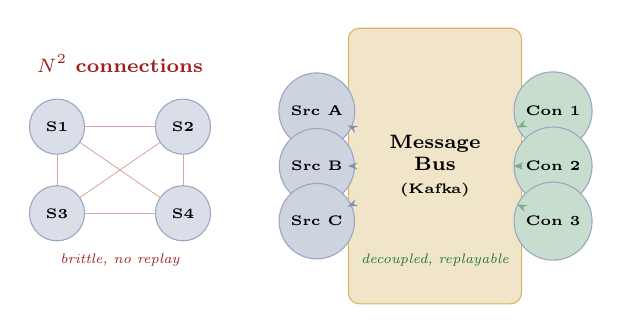
\begin{tikzpicture}[
          sys/.style={circle, draw=PUNavy!40, fill=PUNavy!15,
                      minimum size=0.7cm, font=\tiny\bfseries},
          bus/.style={rectangle, rounded corners=4pt, fill=PUGold!25,
                      draw=PUGold!70, minimum width=2.2cm,
                      minimum height=3.5cm, font=\scriptsize\bfseries,
                      align=center},
          arr/.style={-{Stealth[length=3.5pt]}, thick}
        ]
        % Point-to-point (left)
        \node[font=\scriptsize\bfseries, PURed] at (-2.0, 4.1) {$N^2$ connections};
        \node[sys] (s1) at (-2.8, 3.3) {S1};
        \node[sys] (s2) at (-1.2, 3.3) {S2};
        \node[sys] (s3) at (-2.8, 2.2) {S3};
        \node[sys] (s4) at (-1.2, 2.2) {S4};
        \foreach \a in {s1,s2,s3,s4} {
          \foreach \b in {s1,s2,s3,s4} {
            \draw[PURed!40, very thin] (\a)--(\b);
          }
        }
        \node[font=\tiny\itshape, PURed] at (-2.0, 1.6) {brittle, no replay};

        % Event bus (right)
        \node[font=\scriptsize\bfseries, PUGreen] at (2.0, 4.1) {Event Bus};
        \node[bus] (bus) at (2.0, 2.8) {Message\\Bus\\{\tiny (Kafka)}};
        \foreach \y/\lbl in {3.5/Src A, 2.8/Src B, 2.1/Src C} {
          \node[sys, fill=PUNavy!20] (p\lbl) at (0.5, \y) {\tiny\lbl};
          \draw[arr, PUNavy!50] (p\lbl)--(bus);
        }
        \foreach \y/\lbl in {3.5/Con 1, 2.8/Con 2, 2.1/Con 3} {
          \node[sys, fill=PUGreen!25] (c\lbl) at (3.5, \y) {\tiny\lbl};
          \draw[arr, PUGreen!60] (bus)--(c\lbl);
        }
        \node[font=\tiny\itshape, PUGreen] at (2.0, 1.6) {decoupled, replayable};
      \end{tikzpicture}
      \end{center}
  \end{columns}
\end{frame}

%----------------------------------------------------------------
\begin{frame}{Data Integration Tool Landscape}
  \centering
  \renewcommand{\arraystretch}{1.5}
  \begin{tabular}{p{2.6cm}p{2.0cm}p{2.2cm}p{3.5cm}p{2.2cm}}
    \toprule
    \textbf{Tool} & \textbf{Direction} & \textbf{Type} & \textbf{Primary Use Case} & \textbf{Throughput} \\
    \midrule
    \textbf{Apache Sqoop} &
      RDBMS $\leftrightarrow$ HDFS &
      Batch &
      Nightly bulk transfer of Oracle/MySQL tables to Hadoop &
      GB -- TB/hour \\
    \textbf{Apache Flume} &
      Logs $\to$ HDFS &
      Batch / micro-batch &
      Web server log ingestion; aggregating multi-source logs &
      MB -- GB/hour \\
    \textbf{Apache Kafka} &
      Any $\to$ Any &
      Real-time stream &
      Centralised event bus; fraud events, clickstream, IoT &
      GB -- TB/hour \\
    \textbf{Apache NiFi} &
      Any $\to$ Any &
      Visual pipeline &
      No-code data routing; IoT edge to cloud; file transfer &
      MB -- GB/hour \\
    \textbf{Spark Streaming} &
      Kafka $\to$ HDFS/DB &
      Stream processing &
      Stateful aggregation on streams; enrichment; joins &
      GB/hour \\
    \midrule
    \textbf{Use when} &
      \multicolumn{4}{l}{\small Sqoop = bulk DB sync;\;
        Flume = log collection;\;
        Kafka = real-time events;\;
        NiFi = visual routing;\;
        Spark = stream computation} \\
    \bottomrule
  \end{tabular}
\end{frame}

%================================================================
\section{Batch Integration: Sqoop and Flume}
%================================================================

\begin{frame}{Apache Sqoop: Bulk RDBMS $\leftrightarrow$ HDFS Transfer}
  \begin{columns}[T]
    \column{0.52\textwidth}
      \begin{block}{What Sqoop Does}
        Sqoop (\textbf{SQL-to-Hadoop}) is a command-line tool that transfers data in bulk between a \textbf{relational database} (MySQL, Oracle, PostgreSQL, SQL Server) and \textbf{HDFS} (or Hive, HBase).
        \vspace{4pt}
        \begin{itemize}
          \item \textbf{Import}: copies a table or query result from RDBMS $\to$ HDFS as CSV, Avro, Parquet, or Sequence File
          \item \textbf{Export}: copies data from HDFS $\to$ RDBMS (e.g., after Spark processing, push results back to MySQL)
          \item Internally launches a \textbf{MapReduce job} where each Map task reads a subset of rows (partitioned by primary key range) in parallel
          \item Supports \textbf{incremental import}: only rows newer than the last run (using a \texttt{--last-value} checkpoint on a timestamp or auto-increment column)
        \end{itemize}
      \end{block}
      \begin{exampleblock}{bKash Use Case}
        \small Nightly at 01:00, Sqoop imports the day's bKash wallet transactions (10 M rows) from the production Oracle OLTP database into HDFS as Parquet, partitioned by \texttt{txn\_date}.  Hive analytics then run on HDFS without touching the live database.
      \end{exampleblock}

    \column{0.45\textwidth}
      \begin{center}
      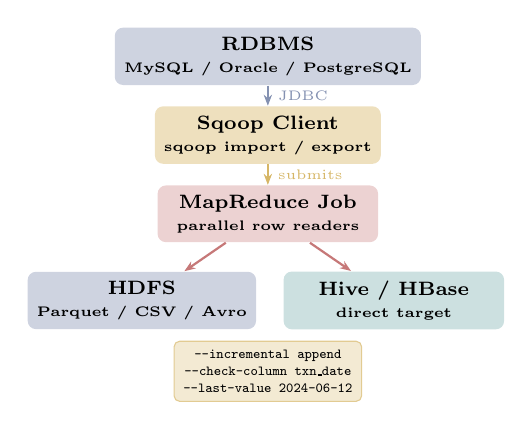
\begin{tikzpicture}[
          box/.style={rectangle, rounded corners=3pt, minimum width=2.8cm,
                      minimum height=0.7cm, font=\scriptsize\bfseries, align=center},
          arr/.style={-{Stealth[length=4pt]}, thick}
        ]
        \node[box, fill=PUNavy!20] (rdb) at (0, 4.6)
              {RDBMS\\{\tiny MySQL / Oracle / PostgreSQL}};
        \node[box, fill=PUGold!30] (sq)  at (0, 3.6)
              {Sqoop Client\\{\tiny sqoop import / export}};
        \node[box, fill=PURed!20]  (mr)  at (0, 2.6)
              {MapReduce Job\\{\tiny parallel row readers}};
        \node[box, fill=PUNavy!20] (hdfs) at (-1.6, 1.5)
              {HDFS\\{\tiny Parquet / CSV / Avro}};
        \node[box, fill=PUTeal!20] (hive) at (1.6, 1.5)
              {Hive / HBase\\{\tiny direct target}};

        \draw[arr, PUNavy!50] (rdb)--(sq)
              node[midway,right,font=\tiny]{JDBC};
        \draw[arr, PUGold!70] (sq)--(mr)
              node[midway,right,font=\tiny]{submits};
        \draw[arr, PURed!60] (mr)--(hdfs);
        \draw[arr, PURed!60] (mr)--(hive);

        % Incremental badge
        \node[rectangle, fill=PUGold!20, draw=PUGold!50, rounded corners=2pt,
              font=\tiny, align=center] at (0, 0.6)
              {\texttt{--incremental append}\\
               \texttt{--check-column txn\_date}\\
               \texttt{--last-value 2024-06-12}};
      \end{tikzpicture}
      \end{center}
  \end{columns}
\end{frame}

%----------------------------------------------------------------
\begin{frame}{Apache Flume: Log Ingestion Pipelines}
  \begin{columns}[T]
    \column{0.52\textwidth}
      \begin{block}{Flume Architecture: Source $\to$ Channel $\to$ Sink}
        Flume moves \textbf{semi-structured log data} (web server logs, application logs, IoT sensor readings) into HDFS for archival and batch analysis.  Every Flume agent has three components:
        \vspace{4pt}
        \begin{itemize}
          \item \textbf{Source}: reads incoming data.  Types: Avro source (from another agent), Syslog source, Exec source (tail a log file), HTTP source
          \item \textbf{Channel}: buffers events between Source and Sink.  Memory channel (fast, no persistence) or \textbf{File channel} (persistent, survives agent restart)
          \item \textbf{Sink}: writes data to the destination.  HDFS sink (writes Avro/text files), Kafka sink (forward to Kafka), HBase sink
        \end{itemize}
        \vspace{4pt}
        Flume supports \textbf{fan-in} (many sources $\to$ one agent) and \textbf{fan-out} (one source $\to$ many sinks) topologies, enabling hierarchical log aggregation across many servers.
      \end{block}

    \column{0.45\textwidth}
      \begin{center}
      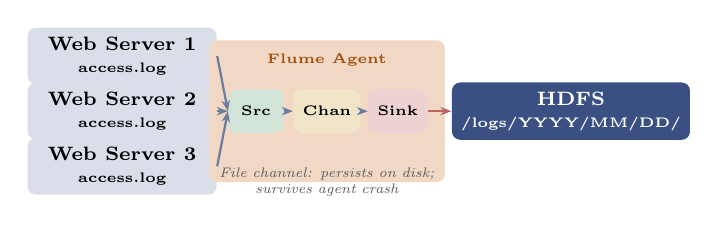
\begin{tikzpicture}[
          comp/.style={rectangle, rounded corners=3pt, minimum width=2.4cm,
                       minimum height=0.65cm, font=\scriptsize\bfseries,
                       align=center},
          arr/.style={-{Stealth[length=4pt]}, thick, PUNavy!60}
        ]
        % Multiple web servers
        \foreach \i/\y in {1/4.4, 2/3.7, 3/3.0} {
          \node[comp, fill=PUNavy!15] (ws\i) at (-2.2, \y)
                {Web Server \i\\{\tiny access.log}};
        }

        % Collector agent
        \node[comp, fill=PUOrange!25, minimum width=3.0cm,
              minimum height=1.8cm] at (0.4, 3.7) {};
        \node[font=\tiny\bfseries, PUOrange!80!black] at (0.4, 4.35)
              {Flume Agent};
        \node[comp, fill=PUGreen!20, minimum width=0.7cm,
              minimum height=0.55cm] (src) at (-0.5, 3.7)
              {\tiny Src};
        \node[comp, fill=PUGold!25, minimum width=0.7cm,
              minimum height=0.55cm] (ch) at (0.4, 3.7)
              {\tiny Chan};
        \node[comp, fill=PURed!20, minimum width=0.7cm,
              minimum height=0.55cm] (sk) at (1.3, 3.7)
              {\tiny Sink};

        \foreach \i in {1,2,3} {
          \draw[arr] (ws\i.east)--(src.west);
        }
        \draw[arr] (src)--(ch);
        \draw[arr] (ch)--(sk);

        % HDFS
        \node[comp, fill=PUNavy!80, text=white, minimum width=2.8cm]
              (hdfs) at (3.5, 3.7) {HDFS\\{\tiny /logs/YYYY/MM/DD/}};
        \draw[arr, PURed!70] (sk)--(hdfs);

        % File channel note
        \node[font=\tiny\itshape, text=PUGray, align=center, text width=2.8cm] at (0.4, 2.8)
              {File channel: persists on disk;\\
               survives agent crash};
      \end{tikzpicture}
      \end{center}
      \vspace{4pt}
      \begin{alertblock}{Flume vs.\ Kafka}
        \small Flume is optimised for \textbf{log collection to HDFS}.  Kafka is a \textbf{general-purpose event bus} with stronger durability and replay semantics.  In modern stacks, Flume is often replaced by Kafka producers writing directly from applications.
      \end{alertblock}
  \end{columns}
\end{frame}

%================================================================
\section{Apache Kafka: The Append-Only Event Log}
%================================================================

\begin{frame}{Apache Kafka: The Core Insight}
  \begin{columns}[T]
    \column{0.52\textwidth}
      \begin{block}{Origin: LinkedIn, 2011}
        LinkedIn needed to move \textbf{activity events} (profile views, connection requests, job clicks, feed impressions) from dozens of producer services to dozens of consumer services (recommendation engines, analytics, monitoring).  Point-to-point messaging created an $N^2$ web of dependencies.

        \vspace{4pt}
        Jay Kreps, Neha Narkhede, and Jun Rao designed Kafka around one insight:
      \end{block}
      \vspace{4pt}
      \begin{alertblock}{The Founding Insight}
        \itshape ``A log is the most primitive form of storage.  If you model your data infrastructure as a distributed, replicated, append-only log, you get \textbf{durability}, \textbf{replayability}, and \textbf{decoupling} for free.''
        \par\hfill --- Kreps, Narkhede \& Rao (2011)
      \end{alertblock}
      \vspace{4pt}
      \begin{exampleblock}{Why ``append-only'' matters}
        \small A traditional queue deletes a message after it is consumed.  Kafka \textbf{retains all messages} for a configurable period (days, weeks, or forever).  Late-joining consumers can read from offset 0 and replay the entire history.  This enables new analytics pipelines to be built without re-ingesting from source.
      \end{exampleblock}

    \column{0.45\textwidth}
      \begin{center}
      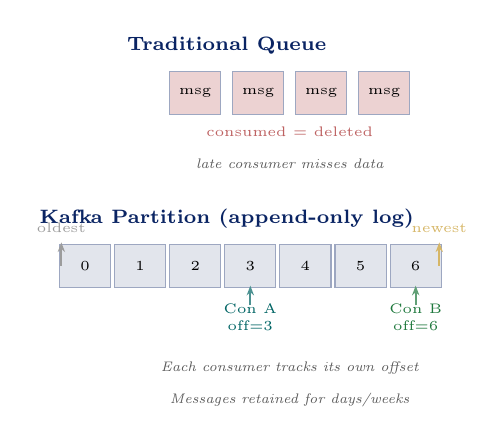
\begin{tikzpicture}[
          rec/.style={rectangle, draw=PUNavy!40, fill=PUNavy!12,
                      minimum width=0.65cm, minimum height=0.55cm,
                      font=\tiny},
          arr/.style={-{Stealth[length=3.5pt]}, thick}
        ]
        \node[font=\scriptsize\bfseries, PUNavy] at (0, 4.5)
              {Traditional Queue};
        \foreach \i/\x in {0/0.0, 1/0.8, 2/1.6, 3/2.4} {
          \node[rec, fill=PURed!20] at (\x-0.4, 3.9) {\tiny msg};
        }
        \node[font=\tiny, PURed!70] at (0.8, 3.4)
              {consumed = deleted};
        \node[font=\tiny\itshape, PUGray] at (0.8, 3.0)
              {late consumer misses data};

        \node[font=\scriptsize\bfseries, PUNavy] at (0, 2.3)
              {Kafka Partition (append-only log)};
        \foreach \off/\x in {0/-1.8, 1/-1.1, 2/-0.4, 3/0.3,
                              4/1.0, 5/1.7, 6/2.4} {
          \node[rec] (k\off) at (\x, 1.7) {\tiny\off};
        }
        \draw[arr, PUGray!60] (-2.1,1.7)--(-2.1,2.0)
              node[above, font=\tiny]{oldest};
        \draw[arr, PUGold!70] (2.7,1.7)--(2.7,2.0)
              node[above, font=\tiny]{newest};

        % Consumer A at offset 3
        \draw[arr, PUTeal!70, thick] (0.3, 1.2)--(0.3, 1.45)
              node[below=3pt, font=\tiny, text=PUTeal, align=center]{Con A\\off=3};
        % Consumer B at offset 6
        \draw[arr, PUGreen!70, thick] (2.4, 1.2)--(2.4, 1.45)
              node[below=3pt, font=\tiny, text=PUGreen, align=center]{Con B\\off=6};

        \node[font=\tiny\itshape, PUGray] at (0.8, 0.4)
              {Each consumer tracks its own offset};
        \node[font=\tiny\itshape, PUGray] at (0.8, 0.0)
              {Messages retained for days/weeks};
      \end{tikzpicture}
      \end{center}
  \end{columns}
\end{frame}

%----------------------------------------------------------------
\begin{frame}{Kafka Architecture: Topics, Partitions, Brokers}
  \begin{columns}[T]
    \column{0.50\textwidth}
      \begin{block}{Key Components}
        {\small
        \begin{itemize}
          \item \textbf{Topic}: a named, durable, append-only log for a category of events (e.g., \texttt{bkash-transactions}, \texttt{pathao-gps-pings})
          \item \textbf{Partition}: each topic is split into $P$ ordered partitions for parallelism.  All messages with the same \textbf{key} go to the same partition (preserving key-level ordering)
          \item \textbf{Offset}: integer index of a message within a partition.  Each consumer independently tracks its own read offset
          \item \textbf{Broker}: a Kafka server that stores partitions on disk.  A cluster has $B$ brokers; each partition has one \textbf{leader} and $R-1$ \textbf{follower replicas} (default $R=3$)
          \item \textbf{Producer}: publishes messages to a topic; selects partition via key hash or round-robin
          \item \textbf{Consumer Group}: a set of consumers that divide a topic's partitions between them for parallel consumption.  Each partition is assigned to exactly one consumer in a group at any time
          \item \textbf{ZooKeeper / KRaft}: manages broker metadata and leader election (ZooKeeper in Kafka $<$3.0; KRaft in Kafka $\geq$3.0)
        \end{itemize}
        }
      \end{block}

    \column{0.47\textwidth}
      \begin{center}
      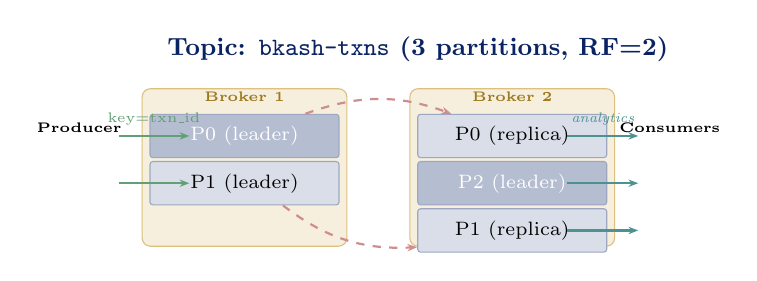
\begin{tikzpicture}[
          part/.style={rectangle, draw=PUNavy!40, fill=PUNavy!12,
                       minimum width=2.4cm, minimum height=0.55cm,
                       font=\scriptsize, rounded corners=1pt},
          brk/.style={rectangle, rounded corners=3pt, draw=PUGold!60,
                      fill=PUGold!15, minimum width=2.6cm,
                      minimum height=2.0cm},
          arr/.style={-{Stealth[length=3.5pt]}, thick}
        ]
        % Topic label
        \node[font=\small\bfseries, PUNavy] at (0.8, 4.6)
              {Topic: \texttt{bkash-txns} (3 partitions, RF=2)};

        % Brokers
        \foreach \b/\x in {1/-1.4, 2/2.0} {
          \node[brk] at (\x, 3.1) {};
          \node[font=\tiny\bfseries, PUGold!80!black] at (\x, 4.0)
                {Broker \b};
        }
        % Partitions: P0 leader on B1, replica on B2
        \node[part, fill=PUNavy!30, text=white]  (p0l) at (-1.4, 3.5) {P0 (leader)};
        \node[part, fill=PUNavy!15]              (p1l) at (-1.4, 2.9) {P1 (leader)};
        \node[part, fill=PUNavy!15]              (p2r) at ( 2.0, 3.5) {P0 (replica)};
        \node[part, fill=PUNavy!30, text=white]  (p2l) at ( 2.0, 2.9) {P2 (leader)};
        \node[part, fill=PUNavy!15]              (p1r) at ( 2.0, 2.3) {P1 (replica)};

        % Replication arrows
        \draw[arr, PURed!50, dashed, bend left=20] (p0l) to (p2r);
        \draw[arr, PURed!50, dashed, bend right=20] (p1l) to (p1r);

        % Producers
        \node[font=\tiny\bfseries] at (-3.5, 3.6) {Producer};
        \draw[arr, PUGreen!70] (-3.0,3.5)--(-2.1,3.5)
              node[midway,above,font=\tiny]{key=txn\_id};
        \draw[arr, PUGreen!70] (-3.0,2.9)--(-2.1,2.9);

        % Consumer Group
        \node[font=\tiny\bfseries] at (4.0, 3.6) {Consumers};
        \draw[arr, PUTeal!70] (2.7,3.5)--(3.6,3.5)
              node[midway,above,font=\tiny\itshape]{analytics};
        \draw[arr, PUTeal!70] (2.7,2.9)--(3.6,2.9);
        \draw[arr, PUTeal!70] (2.7,2.3)--(3.6,2.3);
      \end{tikzpicture}
      \end{center}
  \end{columns}
\end{frame}

%----------------------------------------------------------------
\begin{frame}{Kafka: Throughput, Retention, and Replay}
  \begin{columns}[T]
    \column{0.52\textwidth}
      \begin{block}{How Kafka Achieves High Throughput}
        \begin{itemize}
          \item \textbf{Sequential disk writes}: Kafka never updates messages in place.  Append-only writes are sequential — modern HDDs achieve 600 MB/s sequential vs.\ $<$1 MB/s random.  Kafka exploits this fully.
          \item \textbf{Zero-copy transfer}: Kafka uses the OS \texttt{sendfile()} system call to transfer data from disk to network socket without copying through user-space memory.  Eliminates one full memory copy per message.
          \item \textbf{Batching}: producers and consumers batch multiple messages in one network round-trip.  Configurable via \texttt{batch.size} and \texttt{linger.ms}.
          \item \textbf{Partition parallelism}: $P$ partitions enable $P$ producers and up to $P$ consumers in a group to operate simultaneously — throughput scales linearly with partition count.
        \end{itemize}
      \end{block}

    \column{0.45\textwidth}
      \begin{exampleblock}{Kafka at bKash and Pathao}
        \small \textbf{bKash} uses Kafka topics \texttt{wallet-credit} and \texttt{wallet-debit} to stream every transaction event to three consumers simultaneously:
        \begin{enumerate}
          \item Fraud detection (Spark Streaming, $<$200 ms latency)
          \item Balance update (RDBMS writer)
          \item Audit log writer (HDFS, daily reconciliation)
        \end{enumerate}
        \vspace{4pt}
        \textbf{Pathao} publishes GPS pings every 3 seconds from active drivers to a Kafka topic \texttt{driver-location} (10 partitions, keyed by \texttt{driver\_id}), consumed by the routing engine and the dispatch service independently.
      \end{exampleblock}
      \vspace{4pt}
      \begin{alertblock}{Retention and Replay}
        \small Kafka retains all messages for a configured period (e.g., 7 days) or up to a storage quota.  A new consumer can start at offset 0 and replay the entire week of events --- enabling historical backfill without re-ingesting from the source database.
      \end{alertblock}
  \end{columns}
\end{frame}

%================================================================
\section{Lambda Architecture}
%================================================================

\begin{frame}{Lambda Architecture (Nathan Marz, 2011)}
  \begin{columns}[T]
    \column{0.52\textwidth}
      \begin{block}{Design Goal}
        Serve \textbf{both} accurate historical batch views and \textbf{low-latency} real-time views from the same data, with fault tolerance and the ability to recompute from scratch.
        \vspace{4pt}
        \textbf{Three layers:}
        \begin{enumerate}
          \item \textbf{Batch Layer}: stores the complete, immutable master dataset (HDFS); periodically recomputes \textbf{batch views} (e.g., Spark/Hive jobs running every hour or nightly).  Output is accurate but \textbf{high-latency} (1 hour to 24 hours stale).
          \item \textbf{Speed Layer}: processes new data arriving since the last batch job using a stream processor (Kafka + Spark Streaming / Flink).  Produces \textbf{real-time views} covering the most recent window.  Output is \textbf{approximate but low-latency} ($<$seconds).
          \item \textbf{Serving Layer}: merges batch views and real-time views to answer queries.  A query result = \textit{batch view (up to N hours ago)} UNION \textit{real-time view (last N hours)}.
        \end{enumerate}
      \end{block}

    \column{0.45\textwidth}
      \begin{center}
      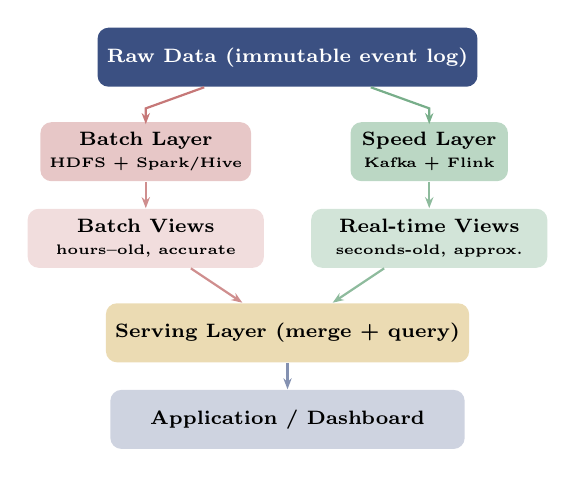
\begin{tikzpicture}[
          box/.style={rectangle, rounded corners=4pt, minimum width=3.0cm,
                      minimum height=0.75cm, font=\scriptsize\bfseries, align=center},
          arr/.style={-{Stealth[length=4pt]}, thick}
        ]
        % Raw data
        \node[box, fill=PUNavy!80, text=white, minimum width=4.5cm]
              (raw) at (0, 5.0) {Raw Data (immutable event log)};

        % Batch layer
        \node[box, fill=PURed!25, minimum width=2.0cm]
              (bl) at (-1.8, 3.8) {Batch Layer\\{\tiny HDFS + Spark/Hive}};
        % Speed layer
        \node[box, fill=PUGreen!30, minimum width=2.0cm]
              (sl) at (1.8, 3.8) {Speed Layer\\{\tiny Kafka + Flink}};

        \draw[arr, PURed!60] (raw)--(-1.8,4.35)--(-1.8,4.15);
        \draw[arr, PUGreen!60] (raw)--(1.8,4.35)--(1.8,4.15);

        % Batch views
        \node[box, fill=PURed!15] (bv) at (-1.8, 2.7)
              {Batch Views\\{\tiny hours--old, accurate}};
        % Real-time views
        \node[box, fill=PUGreen!20] (rv) at (1.8, 2.7)
              {Real-time Views\\{\tiny seconds-old, approx.}};

        \draw[arr, PURed!50]  (bl)--(bv);
        \draw[arr, PUGreen!50] (sl)--(rv);

        % Serving layer
        \node[box, fill=PUGold!35, minimum width=4.5cm]
              (srv) at (0, 1.5) {Serving Layer (merge + query)};
        \draw[arr, PURed!50]  (bv)--(srv);
        \draw[arr, PUGreen!50] (rv)--(srv);

        % Application
        \node[box, fill=PUNavy!20, minimum width=4.5cm]
              (app) at (0, 0.4) {Application / Dashboard};
        \draw[arr, PUNavy!50] (srv)--(app);
      \end{tikzpicture}
      \end{center}
  \end{columns}
\end{frame}

%----------------------------------------------------------------
\begin{frame}{Lambda Architecture: Strengths and Weaknesses}
  \begin{columns}[T]
    \column{0.50\textwidth}
      \begin{exampleblock}{Strengths of Lambda}
        \begin{itemize}
          \item \textbf{Accuracy}: the batch layer always recomputes from raw data, so historical views are correct regardless of bugs or schema changes in earlier runs
          \item \textbf{Low latency}: the speed layer delivers results within seconds for the most recent data window
          \item \textbf{Fault tolerance}: the immutable master dataset on HDFS is the single source of truth; any derived view can be recomputed from it
          \item \textbf{Separation of concerns}: batch and speed components can be built, deployed, and scaled independently
        \end{itemize}
      \end{exampleblock}

    \column{0.47\textwidth}
      \begin{alertblock}{The Critical Weakness: Dual Code Paths}
        Lambda requires implementing \textbf{the same business logic twice}:
        \begin{itemize}
          \item Once in the batch layer (Spark/Hive jobs)
          \item Once in the speed layer (Flink/Spark Streaming)
        \end{itemize}
        \vspace{4pt}
        When business logic changes, \textbf{both implementations must be updated simultaneously and kept in sync}.  Teams report that 30--40\% of engineering effort goes into keeping the two layers consistent --- a significant maintenance burden.
        \vspace{4pt}
        \textbf{Additional complexity:}
        \begin{itemize}
          \item The serving layer must merge two query results at runtime (complex query logic)
          \item Two separate monitoring and debugging pipelines
          \item Two sets of infrastructure (Hadoop cluster + streaming cluster)
        \end{itemize}
      \end{alertblock}
  \end{columns}
\end{frame}

%================================================================
\section{Kappa Architecture}
%================================================================

\begin{frame}{Kappa Architecture (Jay Kreps, 2014)}
  \begin{columns}[T]
    \column{0.52\textwidth}
      \begin{block}{The Simplifying Insight}
        Jay Kreps (co-creator of Kafka) argued that the batch layer in Lambda is unnecessary if your stream processing system is \textbf{powerful enough to reprocess historical data} at the same speed as it processes live data.
        \vspace{4pt}
        \textbf{Kappa's two components:}
        \begin{enumerate}
          \item \textbf{Log storage} (Kafka with long retention or Apache Iceberg on S3): stores the complete immutable event history.  Replacing the HDFS batch layer.
          \item \textbf{Stream processing engine} (Flink, Spark Structured Streaming): the \textbf{single code path} that handles both live events and historical replay.  To reprocess history, start a new consumer at offset 0 and let it catch up.
        \end{enumerate}
        \vspace{4pt}
        \textbf{Reprocessing workflow:}
        \begin{itemize}
          \item Deploy a new version of the stream processing job
          \item Start it from Kafka offset 0 (beginning of history)
          \item It reads and processes all historical events, then seamlessly catches up to live events
          \item When caught up, swap it into production and retire the old version
        \end{itemize}
      \end{block}

    \column{0.45\textwidth}
      \begin{center}
      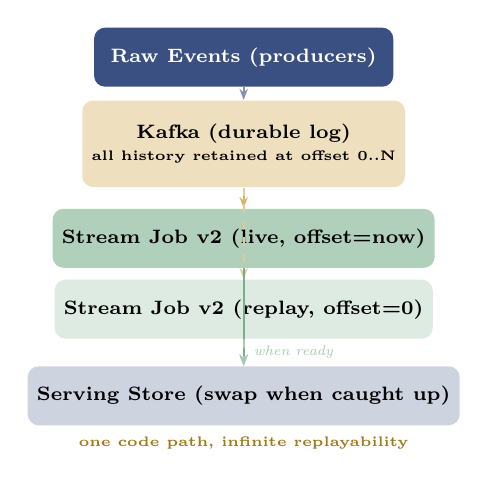
\begin{tikzpicture}[
          box/.style={rectangle, rounded corners=4pt, minimum width=3.8cm,
                      minimum height=0.75cm, font=\scriptsize\bfseries, align=center},
          arr/.style={-{Stealth[length=4pt]}, thick}
        ]
        % Raw events
        \node[box, fill=PUNavy!80, text=white]
              (raw) at (0, 5.0) {Raw Events (producers)};

        % Kafka log
        \node[box, fill=PUGold!30, minimum width=3.8cm,
              minimum height=1.1cm]
              (kaf) at (0, 3.9) {Kafka (durable log)\\{\tiny all history retained at offset 0..N}};

        \draw[arr, PUNavy!50] (raw)--(kaf);

        % Stream job (live)
        \node[box, fill=PUGreen!35]
              (live) at (0, 2.7) {Stream Job v2 (live, offset=now)};
        % Stream job (replay)
        \node[box, fill=PUGreen!15]
              (rply) at (0, 1.8) {Stream Job v2 (replay, offset=0)};

        \draw[arr, PUGold!70] (kaf)--(live);
        \draw[arr, PUGold!50, dashed] (kaf)--(rply);

        % Serving
        \node[box, fill=PUNavy!20]
              (srv) at (0, 0.7) {Serving Store (swap when caught up)};
        \draw[arr, PUGreen!60] (live)--(srv);
        \draw[arr, PUGreen!40, dashed] (rply)--
              node[right,font=\tiny\itshape]{when ready} (srv);

        \node[font=\tiny\bfseries, PUGold!80!black] at (0, 0.1)
              {one code path, infinite replayability};
      \end{tikzpicture}
      \end{center}
  \end{columns}
\end{frame}

%----------------------------------------------------------------
\begin{frame}{Lambda vs.\ Kappa: Full Comparison}
  \centering
  \renewcommand{\arraystretch}{1.5}
  \begin{tabular}{p{3.2cm}p{4.5cm}p{4.5cm}}
    \toprule
    \textbf{Property} & \textbf{Lambda Architecture} & \textbf{Kappa Architecture} \\
    \midrule
    Code paths & Two (batch + stream) — must stay in sync & One (stream only) \\
    Historical reprocessing & Re-run batch job on HDFS & Replay Kafka log from offset 0 \\
    Latency & Low (speed layer) + High (batch layer) & Low throughout \\
    Complexity & High (two systems, merging layer) & Lower (single pipeline) \\
    Batch throughput & Very high (Spark/Hive on full dataset) & Limited by stream engine throughput \\
    Long-term storage & HDFS (immutable master dataset) & Kafka (bounded) + external store (S3/Iceberg) \\
    When to use Lambda & Business logic too complex for stream-only; batch ML training; regulatory batch reports & — \\
    When to use Kappa & Stream engine is fast enough to reprocess; single code path is worth the stream-storage cost & — \\
    \midrule
    \textbf{Kappa NOT suitable when} & \multicolumn{2}{p{9.0cm}}{\small (1) Reprocessing TB+ history is too slow for the stream engine; (2) Batch SQL analytics (Hive, Spark batch) are preferred over stream SQL; (3) Regulatory requirement mandates a separate batch reconciliation system} \\
    \bottomrule
  \end{tabular}
\end{frame}

%================================================================
\section{Data Lakes and the Data Swamp Risk}
%================================================================

\begin{frame}{Data Lake Architecture}
  \begin{columns}[T]
    \column{0.52\textwidth}
      \begin{block}{What Is a Data Lake?}
        A data lake is a centralised repository that stores \textbf{raw data at any scale, in any format} (structured, semi-structured, unstructured) without requiring upfront schema definition.  Data is ingested cheaply and quickly; transformation happens on demand.
        \vspace{4pt}
        \textbf{Four-layer architecture:}
        \begin{enumerate}
          \item \textbf{Ingestion Layer}: Sqoop, Flume, Kafka, NiFi, REST APIs — pulls data from all sources and writes raw files to storage
          \item \textbf{Storage Layer}: HDFS or S3 / Azure ADLS — object storage organised in zones (raw $\to$ processed $\to$ curated)
          \item \textbf{Processing Layer}: Spark, Hive, Presto — transforms and queries data on demand
          \item \textbf{Catalogue / Governance Layer}: Apache Atlas, AWS Glue Data Catalog, Hive Metastore — tracks schemas, lineage, ownership, and access policies
        \end{enumerate}
      \end{block}

    \column{0.45\textwidth}
      \begin{alertblock}{The Data Swamp Problem}
        \small A data lake without governance rapidly becomes a \textbf{data swamp}: raw files accumulate without metadata, owners, or quality guarantees.  Symptoms:
        \begin{itemize}
          \item Analysts cannot find relevant datasets (no catalogue)
          \item No one knows which files are current vs.\ stale
          \item Multiple copies of the same data with different transformations exist with no version control
          \item PII (personal data) is mixed with non-sensitive data, violating privacy regulations
        \end{itemize}
        \vspace{4pt}
        \textbf{Prevention:} enforce a data catalogue at ingest time; assign owners to every dataset; implement access control; run automated quality checks; use a table format (Delta Lake, Apache Iceberg) to add ACID guarantees to the lake.
      \end{alertblock}
  \end{columns}
\end{frame}

%================================================================
\section{Ivy League Alignment}
%================================================================

\begin{frame}{Pipelines \& Architectures in Top University Curricula}
  \begin{columns}[T]
    \column{0.55\textwidth}
      \begin{block}{MIT 6.830 — Database Systems}
        \small MIT frames the Lambda and Kappa architectures as answers to a classical database question: \textbf{how do you serve both OLAP (batch analytics) and OLTP (real-time transactions) from the same data?}
        \begin{itemize}
          \item Lambda = a distributed version of the classical data warehouse + OLTP dual architecture
          \item Kappa = a stream-first architecture that eliminates the data warehouse entirely, replacing it with a replayable log
          \item MIT students implement a mini Kafka (topics, partitions, producers, consumers) from scratch in Go as a course project — reinforcing that the append-only log is the fundamental primitive, not a specific product
        \end{itemize}
        \textbf{MIT exam question:} \textit{``Why does Kafka use sequential disk writes rather than a B-tree index?  Quantify the throughput difference on spinning disk.''}
      \end{block}

    \column{0.42\textwidth}
      \begin{exampleblock}{Stanford CS246 — Mining Massive Datasets}
        \small Stanford covers Kafka as the canonical example of \textbf{durable, replayable distributed log storage} — the same abstraction as Google's distributed log (used internally in Google's Spanner and BigTable replication).  CS246 uses Kafka + Spark Structured Streaming as the lab environment for real-time PageRank computation on a Twitter follow graph.
      \end{exampleblock}
      \vspace{4pt}
      \begin{alertblock}{CMU 15-721 — Advanced DB Systems (Pavlo)}
        \small CMU compares Kafka's log-structured storage to LSM-trees (Log-Structured Merge trees) used in RocksDB, Cassandra, and HBase --- all exploit sequential writes for high throughput.  CMU 15-721 covers the \textbf{Lakehouse} pattern (Delta Lake + Spark + Kafka) as the convergence of data lake and data warehouse, previewing Week 11 of this course.
      \end{alertblock}
  \end{columns}
\end{frame}

%================================================================
\section{Student Assessment Pool}
%================================================================

\begin{frame}{Assessment\textemdash MCQ Set A \hfill\small\textit{CLO3, CLO4}}
  \begin{exampleblock}{Instructions}
    Select the single best answer.  Correct answers \textbf{bolded} for instructor reference.
  \end{exampleblock}
  \vspace{6pt}
  \begin{itemize}
    \item[\textbf{Q1.}] Which tool is specifically designed to transfer data in bulk between an RDBMS (e.g., MySQL) and HDFS?
    \begin{enumerate}[(a)]
      \item Apache Flume
      \item Apache Kafka
      \item \textbf{Apache Sqoop}
      \item Apache NiFi
    \end{enumerate}
  \end{itemize}
  \vspace{8pt}
  \begin{itemize}
    \item[\textbf{Q2.}] Apache Kafka's data model is based on which fundamental storage abstraction?
    \begin{enumerate}[(a)]
      \item B-tree indexes for fast point lookups
      \item Column-family storage (like HBase)
      \item \textbf{Append-only immutable distributed logs (partitioned topics)}
      \item Document storage with secondary indexes
    \end{enumerate}
  \end{itemize}
  \vspace{6pt}
  \begin{alertblock}{Instructor Notes}
    \textbf{Q1:} Flume (a) is for logs to HDFS; Kafka (b) is for real-time streaming; NiFi (d) is a visual pipeline tool.  Only Sqoop (c) uses JDBC to do parallel RDBMS $\leftrightarrow$ HDFS bulk transfer.  \textbf{Q2:} The append-only log is the most important conceptual distinction --- Kafka never updates or deletes a message; it only appends.  This enables the replay property that distinguishes Kafka from traditional queues.
  \end{alertblock}
\end{frame}

%----------------------------------------------------------------
\begin{frame}{Assessment\textemdash MCQ Set B \hfill\small\textit{CLO3, CLO4}}
  \vspace{6pt}
  \begin{itemize}
    \item[\textbf{Q3.}] In the Lambda architecture, which layer handles \textbf{real-time, low-latency} query views?
    \begin{enumerate}[(a)]
      \item Batch Layer \quad (b) Serving Layer \quad (c) \textbf{Speed Layer} \quad (d) Ingestion Layer
    \end{enumerate}
  \end{itemize}
  \vspace{8pt}
  \begin{itemize}
    \item[\textbf{Q4.}] The Kappa architecture differs from the Lambda architecture primarily by:
    \begin{enumerate}[(a)]
      \item Adding a third processing layer for machine learning
      \item Using only relational databases for both batch and stream storage
      \item \textbf{Eliminating the batch layer and using Kafka log replay for all reprocessing}
      \item Replacing Hadoop with Spark in the batch layer while keeping the speed layer
    \end{enumerate}
  \end{itemize}
  \vspace{6pt}
  \begin{alertblock}{Instructor Notes}
    \textbf{Q3:} The Serving Layer (b) is not a processing layer --- it merges precomputed views and serves queries.  The Batch Layer (a) is high-latency.  The Speed Layer (c) is the real-time component.  \textbf{Q4:} Option (d) is a common misconception --- Kappa does not just replace Hadoop; it eliminates the entire batch layer and relies on a single stream processing code path with log replay for historical reprocessing.
  \end{alertblock}
\end{frame}

%----------------------------------------------------------------
\begin{frame}{Assessment\textemdash True / False \hfill\small\textit{CLO3}}
  \begin{block}{Instructions}
    State True or False and provide a \textbf{one-sentence justification} for full marks.
  \end{block}
  \vspace{4pt}
  \centering
  \renewcommand{\arraystretch}{1.6}
  \begin{tabular}{p{9.0cm}c}
    \toprule
    \textbf{Statement} & \textbf{Answer} \\
    \midrule
    1.\ Apache Sqoop is designed for real-time streaming ingestion from transactional systems. &
    \alert{\textbf{False}} \\
    2.\ Kafka retains messages for a configurable period, allowing consumers to replay events from any past offset. &
    \textbf{True} \\
    3.\ The Lambda architecture requires maintaining two separate code paths implementing the same business logic. &
    \textbf{True} \\
    4.\ Apache Flume is the preferred tool for collecting and aggregating server log data into HDFS. &
    \textbf{True} \\
    \bottomrule
  \end{tabular}
  \vspace{6pt}
  \begin{exampleblock}{Model Justifications}
    \small \textbf{1:} Sqoop is a \textbf{batch} tool that launches MapReduce jobs for bulk RDBMS$\leftrightarrow$HDFS transfers, typically scheduled nightly.  For real-time ingestion, Kafka is the appropriate tool.  \textbf{3:} Lambda's batch layer and speed layer must both implement the same aggregation logic (e.g., daily transaction count) --- one in Spark batch (HiveQL/SQL) and once in Spark Streaming / Flink (streaming SQL).  This dual maintenance is the architecture's primary engineering cost.
  \end{exampleblock}
\end{frame}

%----------------------------------------------------------------
\begin{frame}{Assessment\textemdash Descriptive Questions \hfill\small\textit{CLO3}}
  \begin{block}{Instructions}
    Answer each question in \textbf{100--150 words}.  Include a diagram where indicated.
  \end{block}
  \vspace{8pt}
  \begin{itemize}
    \item[\textbf{D1.}] Explain the \textbf{Lambda architecture} with a labelled diagram.  What are its three layers?  What is its primary engineering disadvantage compared to the Kappa architecture?
  \end{itemize}
  \vspace{8pt}
  \begin{itemize}
    \item[\textbf{D2.}] Describe how Apache Kafka achieves \textbf{high throughput and fault tolerance}.  Explain the roles of topics, partitions, offsets, brokers, and replication factor in the Kafka data model.
  \end{itemize}
  \vspace{8pt}
  \begin{itemize}
    \item[\textbf{D3.}] What is a \textbf{data lake}?  How does it differ from a data warehouse in terms of schema enforcement, storage format, and typical use cases?  What is a ``data swamp'' and how is it prevented?
  \end{itemize}
\end{frame}

%----------------------------------------------------------------
\begin{frame}{Assessment\textemdash Analytical Questions \hfill\small\textit{CLO4}}
  \begin{block}{Instructions}
    Answer in \textbf{200--300 words} with step-by-step reasoning and tool justifications.
  \end{block}
  \vspace{6pt}
  \begin{itemize}
    \item[\textbf{A1.}] \textbf{Pipeline Design for a Bank:}\\
    Design a data integration pipeline for a Bangladeshi commercial bank that must:
    \begin{itemize}
      \item (a) Synchronise 10 million customer records nightly from Oracle to Hadoop for analytics
      \item (b) Detect fraudulent card-swipe events in real time with a decision within 200 ms
      \item (c) Power a risk management dashboard with data no older than 5 minutes
    \end{itemize}
    Specify which tool (Sqoop, Flume, Kafka, Spark Streaming) you would use at each stage.  Justify each choice with reference to latency, throughput, and fault-tolerance requirements.  Which architecture (Lambda or Kappa) fits best, and why?
  \end{itemize}
  \vspace{6pt}
  \begin{itemize}
    \item[\textbf{A2.}] \textbf{Lambda to Kappa Migration:}\\
    A team using Lambda architecture complains that maintaining two code paths (batch + stream) doubles development cost.  Their CTO suggests migrating to Kappa.  Analyse: (a) what must be true about the stream processing engine for Kappa to be viable; (b) what are the risks of migrating; (c) under what conditions is Kappa \textbf{not suitable} (give at least two concrete scenarios from the Bangladesh financial or healthcare sector)?
  \end{itemize}
\end{frame}

%================================================================
\section*{Textbook References}
%================================================================

\begin{frame}{Textbook \& Reading References}
  \begin{block}{Primary Textbooks for Week 8}
    \begin{itemize}
      \item \textbf{[TW]}\ Tom White. \textit{Hadoop: The Definitive Guide}, O'Reilly, 4th ed., 2015.
            \hfill \textbf{Ch.\ 14, 15}
            \begin{itemize}
              \small\item Ch.\,14: Apache Flume — architecture, sources, channels, sinks, fan-in/fan-out
              \item Ch.\,15: Apache Sqoop — import/export, incremental, partitioning
            \end{itemize}
      \item \textbf{[SA]}\ Acharya \& Chellappan. \textit{Big Data and Analytics}, Wiley, 2015.
            \hfill \textbf{Ch.\ 8}
            \begin{itemize}
              \small\item Ch.\,8: Data integration tools and architectures overview
            \end{itemize}
      \item \textbf{[TE]}\ Erl, Khattak \& Buhler. \textit{Big Data Fundamentals}, Prentice Hall, 2016.
            \hfill \textbf{Ch.\ 10}
            \begin{itemize}
              \small\item Ch.\,10: Big Data integration patterns and enterprise architecture considerations
            \end{itemize}
    \end{itemize}
  \end{block}
  \vspace{4pt}
  \begin{exampleblock}{Graduate Reference and Seminal Paper (covered in Week 8, Part 2)}
    \begin{itemize}
      \small
      \item Kreps, J., Narkhede, N., \& Rao, J.\ (2011). \textbf{Kafka: A Distributed Messaging System for Log Aggregation.} LinkedIn Engineering. [PRIMARY SEMINAL PAPER]
      \item Kleppmann, M.\ (2017). \textit{Designing Data-Intensive Applications.} O'Reilly. Ch.\,3 (storage engines), Ch.\,10 (batch processing), Ch.\,11 (stream processing). [Graduate-level systems reference at MIT, CMU, Stanford]
    \end{itemize}
  \end{exampleblock}
\end{frame}

%----------------------------------------------------------------
\begin{frame}[c]
  \begin{center}
    {\Large\bfseries Questions \& Discussion}\\[10pt]
    {\large Week 8, Part 1 $\;\mid\;$ CSE 4345 Big Data Analytics}\\[8pt]
    \textcolor{PUGray}{\rule{7cm}{0.5pt}}\\[10pt]
    \begin{quote}
      \itshape ``I believe that a unified log is the central data structure that can solve the coherency problem in a distributed, heterogeneous data system \textemdash\ a structure so simple that we take it for granted, and so fundamental that we underestimate it.''
    \end{quote}
    \hfill\textemdash\ Jay Kreps, \textit{The Log}, LinkedIn Engineering, 2013
    \vspace{12pt}
    \begin{block}{\centering Next Lecture: Week 8, Part 2}
      \centering
      Seminal Paper: Kreps, Narkhede \& Rao (2011) --- \textit{``Kafka: A Distributed Messaging System for Log Aggregation''}\\[4pt]
      \small Case Study: \textbf{Netflix Keystone Real-time Stream Processing Platform} ---
      500 billion events per day, Kafka + Flink + S3 + Apache Iceberg
    \end{block}
    \vspace{6pt}
    \textbf{Reading before Part 2:}\ \textbf{[TW]} Ch.\,14--15 $\cdot$ Kreps et al.\ (2011) Kafka paper (see references)
  \end{center}
\end{frame}

%=================================================================
\end{document}
%=================================================================
